% See http://tex.stackexchange.com/questions/168169/options-for-supplementary-materials-in-preprint-version-revtex-arxiv

\pagebreak
\begin{center}
\textbf{\large Supplemental Materials}
\end{center}

\setcounter{equation}{0}
\setcounter{figure}{0}
\setcounter{table}{0}
% \setcounter{page}{1}
\makeatletter
\renewcommand{\theequation}{S\arabic{equation}}
\renewcommand{\thefigure}{S\arabic{figure}}
% \renewcommand{\bibnumfmt}[1]{[S#1]}
% \renewcommand{\citenumfont}[1]{S#1}

Data and notebooks for these analyses are available at \url{https://github.com/hammerlab/XXX}

\begin{figure}
\centering
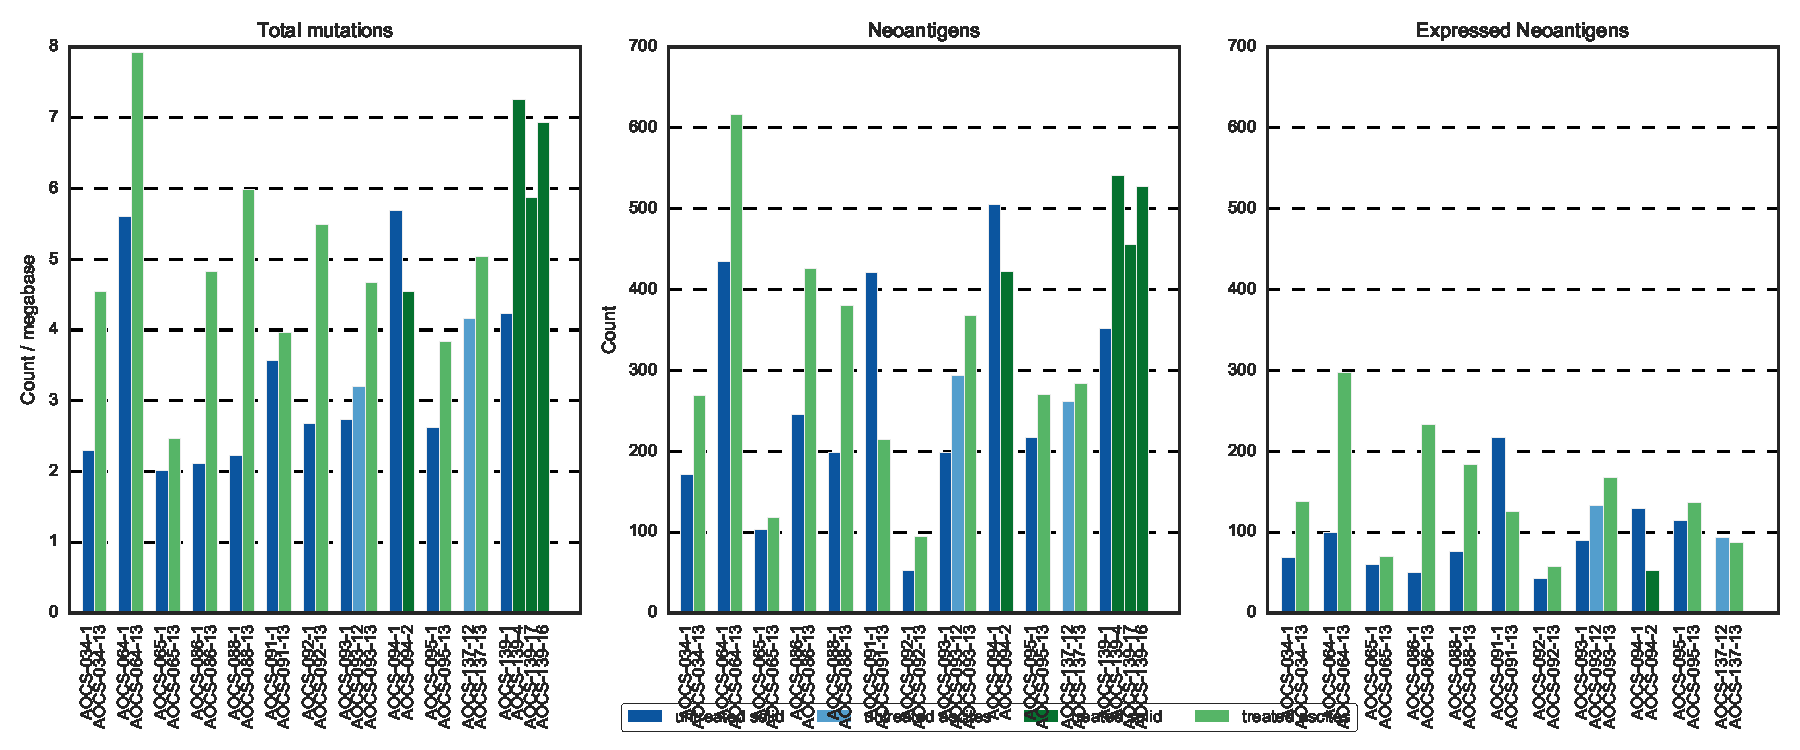
\includegraphics[scale=1.0]{figures/paired_counts.pdf}
\caption{Paired counts. }
\label{sfig:supp_paired}
\end{figure}

\begin{figure}
\centering
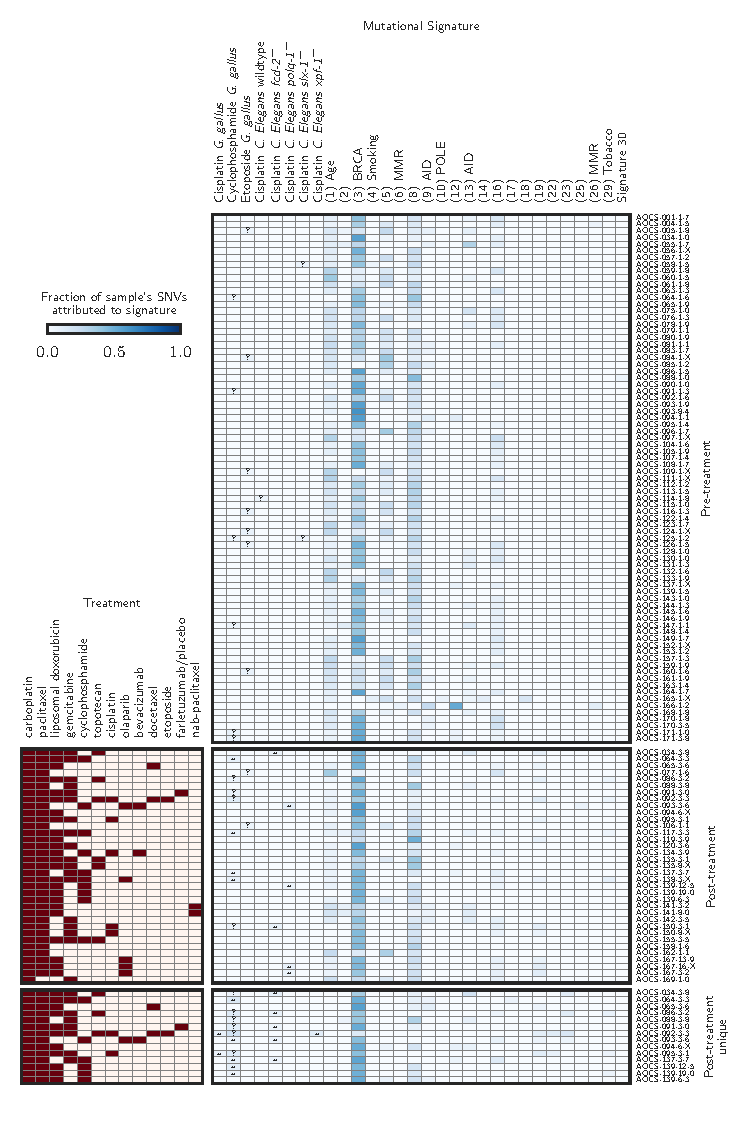
\includegraphics[scale=1.0]{figures/supplementary_signatures.pdf}
\caption{Mutational signature deconvolution for all AOCS samples. }
\label{sfig:supp_signatures}
\end{figure}

\begin{figure}
\centering
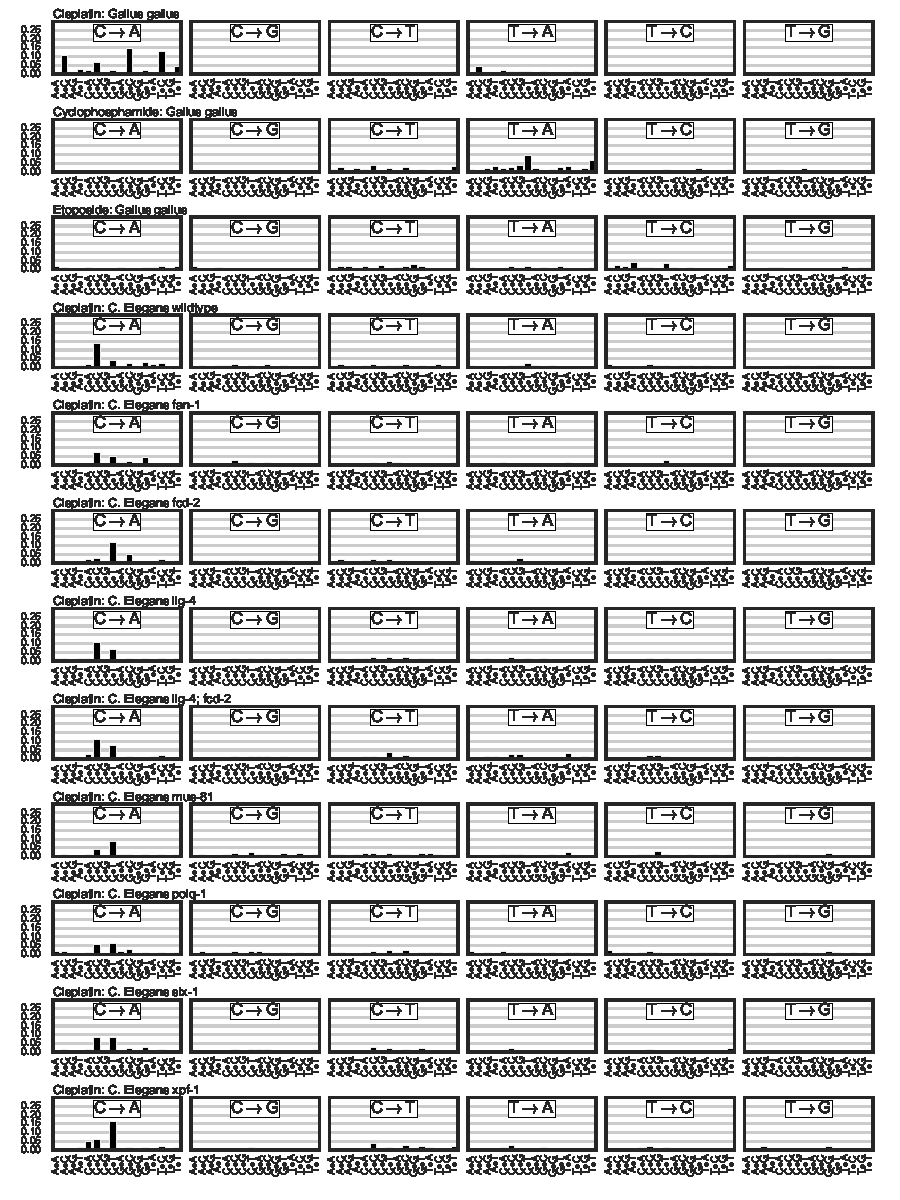
\includegraphics[scale=1.0]{figures/extracted_signatures.pdf}
\caption{Extracted signatures. }
\label{sfig:supp_extracted_signatures}
\end{figure}

\FloatBarrier
